\section{Beschneidung des Netzes zur Beschleunigung des Training}
Das Beschneiden\footnote{Beschneiden wird hier equivalent zum Englischen  "`to prune"' verwendet} des Netzes ist eine Technik, die entwickelt wurde, um die Inferenzzeit eines neuronalen Netzwerks zu reduzieren. Das Beschneidungsverfahren wird auf das bereits trainierte Netz angewendet. Dabei wird entschieden, welche Gewichte nur einen minimalen oder keinen Effekt auf das Klassifikationsergebnis haben, um diese zu entfernen.

Das Beschneiden des Netzes kann auch verwendet werden, um die Trainingszeit zu minimieren. Diese Methode soll in diesem Unterkapitel erläutert werden. Als Quelle für dieses Unterkapitel dient ein Paper, welches evaluiert in wiefern Trainingszeit mittels Beschneiden gespart werden kann \cite{prunetrain}.


Das Ziel des Beschneidens währenddem Training ist es, die Gewichte einzelner Kanäle auf Null zu setzen und zu entfernen, um mit einem kleinerem Netz in den nachfolgenden Epochen Trainingszeit zu sparen. Dazu wird der Loss-Funktion des Netzwerks ein Normalisierungsterm addiert. Damit die Gewichte ganzer Kanäle möglichst unter den Threshold fallen werden die Gewichte der Kanäle gemeinsam quadriert, wie in der folgenden Gleichung zu sehen ist:

\begin{equation}
GL(\bigcup_{l=1}^{L} W_{:,:,:,:}^{(l)})=\sum_{l=1}^{L} \left( \sum_{c_l=1}^{C_l} || W_{c_l,:,:,:}^{(l)} ||_2 + \sum_{k_l=1}^{K_l} || W_{:,k_l,:,:}^{(l)}||_2 \right)
 \label{equ:PTloss}
\end{equation}

Dieser Term nennt sich Group-Lasso. Der Parameter $W_{:,:,:,:}^{(l)}$ stellt die Gewichte im CNN als Tensor dar. Mit $l$ wird dargestellt um welches Layer es sich handelt. Die Dimensionen des Tensors sind: Ausgangskanäle \texttimes Eingangskanäle \texttimes Kerneldimension 1 \texttimes Kerneldimension 2. $L$ gibt an über wieviele Layer der Group-Lasso Term berechnet wird. $k_l$ ist die Laufvariable über die einzelnen Eingangskänale und $c_l$ über die einzelnen Ausgangskanäle.

Um das Verhältnis von Group-Lasso Term zur Loss-Funktion dynamischer wählen zu können, werden diese nicht einfach aufeinander addiert. Es wird abhängig von der Initialbelegung der Gewichte ein Parameter $\lambda$  berechnet, der Group-Lasso und Loss-Funktion balanciert:

\begin{equation}
 LPR(GL(\bigcup_{l=1}^{L} W_{:,:,:,:}^{(l)}),l(y_i,f(x_i,W))) = \frac{\lambda \cdot GL(\bigcup_{l=1}^{L} W_{:,:,:,:}^{(l)})}{l(y_i,f(x_i,W)) + \lambda \cdot GL(\bigcup_{l=1}^{L} W_{:,:,:,:}^{(l)})}           
\end{equation}

Die Größe LPR ist hier echt zwischen Null und Eins wählbar. Je größer sie gewählt wird, desto größer ist der Anteil, der beschnitten wird. Regelmässig werden währenddem Trainieren des Netzes Gewichte, die unter dem Threshold liegen auf Null gesetzt. Es entsteht ein nur dünn besetztes Netz. 



\todo[inline]{Grafik} Gewichte, die unter dem Threshold liegen sind in einer anderen Farbe markiert.
 

 Dann wird durch ein Rekonfigurationsverfahren aus dem Sparse Netz ein Dense Netz ohne die vorher nicht besetzten Kanäle. Um dieses Verfahren durchzuführen muss überprüft werden, ob mit dem Entfernen der Kanäle die Dimensionen der verschiedenen aufeinanderfolgenden Kanäle übereinstimmen. Bei einem residualen Netz muss zusätzlich darauff geachtet werden, dass die Dimensionen der Kurzschluss-Verbindungen zusammen passen.


Zu desem Zweck wird das Channel-Union Verfahren eingeführt. Beim Channel Union Verfahren wird ein Liste mit den Layern geführt, die aufeinander abgestimmt werden müssen. Im Falle eines residualen Netzes muss zusätzlich eine Liste über die zusammengehörigen Layer der Kurzschlussverbindungen geführt werden. Im nächsten Schritt werden alle Eingangs- und Ausgangskanäle, die noch Gewichte größer Null haben in einer Liste gesammelt. Auf allen Elementen dieser Liste wird nun geprüft, ob mit Hilfe von Vereinigungen Kanäle gefunden werden können die zwar keine von Null verschiedenen Gewichte mehr haben, wegen der Dimensionalität aber trotzdem beibehalten werden müssen. Alle Kanäle die nicht unter diese Bedingung fallen können mit Hilfe einer Rekonfiguration aus dem Netzwerk entfernt werden. 
\todo[inline]{Beispiel für Channel Union?}
Bei einem residualen Netzwerk ist es weiterhin möglich, dass ein ganzer Block wegfällt. In diesem Fall müssen die Chanell-Union Listen angepasst werden und es wird mit einem ohne diesen Block um mehrere Layer verkürztes Netzwerk weitergemacht.


Da mit dem Verkleinern des Netzes nicht nur potentiell Zeit sondern auch Speicherplatz gespart wird, kann bei gleicher Speicherauslastung die Batchgröße erhöht werden. Hierbei wird die Lernrate an die erhöhte Batchgröße angepasst um negative Effekte für die Accuracy abzumildern oder auszuschliessen. 

Damit lassen sich Netzverkleinerungs-Raten von etwa 50 \% Erreichen bei weniger als 2 \% Accuracy-Verlust. Andere Techniken schaffen zwar zwischen 70 - 80 \% Netzverkleinerungsraten brauchen aber wesentlich mehr Trainingszeit \cite{lottery}. Diese großen Verkleinerungsraten sind dort sehr stark abhängig von der Initialisierung \cite{lottery}. Das heißt nur einzelne Initialisierungen führen zu so starken Verkleinerungsraten, was insgesamt zu einer längeren Trainingszeit führt \cite{lottery} 




\section{Beschleunigung des Lernens durch Wissenstransfer}
\color{blue1}
Beim Trainieren eines CNNs kommt es häufig vor, dass nach initialem Wählen der Tiefe bzw. Breite des Netzes diese Parameter in einem weiteren Trainingslauf erhöht werden und in Folge dessen das Netzwerk komplett neu trainiert werden muss. Mit Hilfe der Quelle zu diesem Unterkapitel wurde ein Verfahren geschaffen, welches das Netz tiefer oder breiter machen kann und dabei die im ersten Trainingsdurchlauf trainierten Gewichte weiter verwendet \cite{net2net}. Durch diesen Wissenstransfer von einem Netz zu einem tieferen oder breiteren Netz wird eine schnellere Konvergenz des neuen Netzes erwartet. Durch die Initialisierung mit schon vorhandenen Parametern entsteht eine Transformation, die die erlernte Funktion erhält.

\begin{figure}[h]
 \centering
 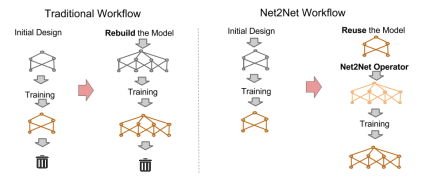
\includegraphics[width=0.7\textwidth]{KapitelPartA/images/net2net.png}
 % net2net.png: 433x179 px, 72dpi, 15.28x6.31 cm, bb=0 0 433 179
 \caption{Traditioneller Workflow vs. Net2Net Workflow}
 \label{abb:net2net}
\end{figure}


Wie in Abbildung \ref{abb:net2net} abgebildet ist lässt sich so der Workflow zum Finden der passenden Netzstruktur anders gestalten. Der Net2Net Operator macht dabei das Netz entweder breiter (mehr Kanäle in bestimmten Schichten) oder tiefer (zusätzliche Schichten). Diese beiden Operatoren werden nun vorgestellt.

\subsection{Operator für breiteres Netz}
\color{blue1}
Bei dem Net2Net-Operator, der das Netz breiter macht werden für eine bestimmte Schicht Ausgangskanäle und für die nachfolgende Schicht Eingangskanäle hinzugefügt. Die Schicht, der Ausgangskanäle hinzugefügt werden wird mit $i$ bezeichnet und hat den Gewichtstensor $\mathbf{W}^i$ mit der Dimensionalität von $c_n \times k_l \times f_1 \times f_2$. Die Schicht, der Eingangskanäle hinzugefügt werden wird mit $i+1$ bezeichnet und hat den Gewichtstensor $\mathbf{W}^{i+1}$ mit der Dimensionalität von $c_m \times k_n \times f_3 \times f_4$. Dem Layer $i$ werden $q$ Kanäle hinzuefügt. Dies entspricht wie in Abbildung \ref{abb:channels} abgebildet ist $q \cdot l $ zusätzlichen Filterkerneln. 

\begin{figure}[h]
 \centering
 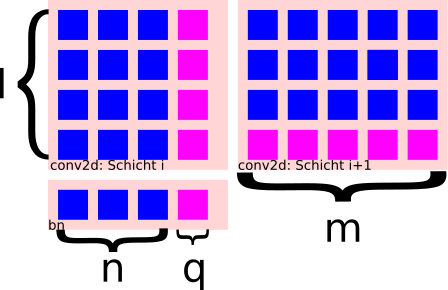
\includegraphics[width=0.6\textwidth]{KapitelPartA/images/channels.png}
 % channels.pdf: 0x0 px, 300dpi, 0.00x0.00 cm, bb=
 \label{abb:channels}
 \caption{Übersicht über die zusätzlichen Kanäle todo: Grafik schön machen}
\end{figure}



Für das Layer $i+1$ sind es entsprechend $q \cdot m $ zusätzliche Kernel. Die Gewichtstensoren nachdem Anwenden des Net2Net Operators werden mit $\mathbf{U}^i$ und $\mathbf{U}^{i+1}$ bezeichnet und sollen die Dimensionalität von $\mathbf{U}^i: c_{n+q} \times k_l \times : \times :$ und $\mathbf{U}^{i+1}: c_m \times k_{n+q} \times : \times :$ haben. Der Net2Net Operator wird angewendet, indem zunächst eine Mapping Funktion $g$ definiert wird die für ein zufällige Belegung der zusätzlichen Kernels sorgt:

\begin{equation}
 g_{j} =  
 \begin{cases}
 j & , \text{ falls} \, j \leq n \\
 k & , \text{ falls} \, j>n : \;  k \text{ zufälliges Sample von} \left\{ 1,2,\ldots, n \right\} \\ 
 \end{cases} 
 \end{equation}
 Mit Hilfe dieser Mapping-Funktion werden nun die neuen Gewichtstensoren initialisiert:
 \begin{equation}
 \mathbf{U}^i_{j,k,f_1,f_2} = \mathbf{W}^i_{g(j),k,f_1,f_2} \; \; \mathbf{U}^{i+1}_{h,j,f_3,f_4}= \frac{1}{|\left\{ x | g(x)=g(j)\right\}|}\mathbf{W}^{i+1}_{h,g(j),f_3,f_4}
 \end{equation}
Die Funktion $g(j)$ wird dabei für jede neu hinzugekommene Schicht nur einmal ausgewertet, sodass gesamte Reihen statt einzelne Kernel kopiert werden. Sollte sich zwischen dem $i$-ten und $(i+1)$-Layer eine Batchnormalisierung befinden, so werden die Parameter dieser Schicht ebenfalls kopiert.

Um nicht mehrere exakt gleiche Kernelreihen zu haben kann ausserdem noch ein Noiseanteil auf alle neuen Gewichte addiert werden. Dies ist vorallem für den Fall wichtig, wenn der Trainingsalgorithmus keine Form der Randomiesierung hat, die gleichen Gewichtstensoren ermutigt unterschiedliche Funktionen zu erlernen. Somit sind die vom ursprünglichen und neuen Netz gelernten Funktionen ähnlich aber nicht gleich.

\subsubsection{Tieferes Netz}

Der Net2Net- Operator für ein tiefers Netz ersetzt die Operation des $i$-ten Layers $\mathbf{h}^{(i)} = \phi\left(\mathbf{h}^{(i-1)t} \mathbf{W}^{(i)}\right)$ durch die Operation von zwei Layern  $\mathbf{h}^{(i)} = \phi( \mathbf{U}^{(i)t} \phi(\mathbf{W}^{(i)t}  \mathbf{h}^{(i-1}) )$. $\mathbf{U}$ wird als Identitätsmatrix initialisiert. Um die geforderte Erhaltung der gelernten Funktion zu erhalten muss für die Aktivierungsfunktion $\phi$ und alle Vektoren $\mathbf{v}$ die Gleichung $\phi(\mathbf{I} \phi(\mathbf{v}))=\phi(\mathbf{v}))$. Die Aktivierungsfunktion ReLu erfüllt diese Anflorderung.

Wird zwischen den beiden Layern eine Batchnormalisierung genutzt, so müssen die Parameter der Batchnormalisierung so gewöhlt werden, dass sie die gelernte Funktion des Netzes nicht verändert.


\subsubsection{Diskussion der Methode}

Die beiden Net2Net-Operatoren schaffen die Möglichkeit Familien von Netzarchitekturen zu erforschen ohne jedes Mal von neuem zu lernen. Mit Hilfe der eiden Operatoren lässt sich die Komplexität des Netzes erhöhen ohne die gelernte bisherige Funktion zu vernachlässigen.


\section{Schnelles Ressourcen beschränktes Strukturlernen tiefer Netzwerke}
Im Gegensatz zu den beiden vorherigen Kapiteln, in denen jewels eine Möglichkeit ein CNN kleiner sowie größer zu machen vorgestellt wurden geht es jetzt darum dies zu kombinieren. Die Quelle für diese Kapitel ist soweit nicht anders gekennzeichnet  das Paper, welches die Methode vorgestellt hat \cite{morphnet}.

Die manuelle Wahl von Hyperparametern, die bestimmen wie gross und komplex ein neuronales Netz ist, braucht eine gewisse Kunstfertigkeit. Sind die Hyperparameter falsch gewählt, so müssen diese angepasst und das Netz erneut trainiert werden. Mit Hilfe der hier vorgestellten Methode wird diese Prozedur automatisiert. Nach einmal gewählten Hyperparametern wird das Netz so angepasst, dass 


Zunächst werden getrennt die hier verwendeten Methoden um das Netz grösser und kleiner zu machen vorgestellt, bevor diese zu einer Methode kombiniert werden.

